%************************************************
\chapter{Design and implementation}\label{ch:design}
%************************************************

%TODO resumir organización del capítulo

% Estructura:
% +Design
%  -Architecture design: delegation, computation offloading, duality User/SC + Engine
% 
% +Implementation:
%  -REST as current delegation protocol.
%  -BIOSC as current APDU transmission protocol: no security -> no overload.
%  -IoT Smart Card software design and implementation notes.
%  -Sequence diagrams. TODO

In this chapter we will describe the process for defining how a constrained IoT device may be integrated in a system like P2ABCE. We will also describe the PoC implementation carried out to test a realistic deployment.

\section{Design}

In this section we will define how an IoT device may be integrated in the P2ABCE architecture, being totally compatible with any other system using P2ABCE, addressing the power and memory constrains many IoT devices face.

We decided to use P2ABCE with the Idemix as its Engine, because it is officially supported by the Idemix Library, it has the most up-to-date implementation, as we saw in the state of the art, and adds capabilities to Idemix like the Presentation Policies, or interoperability with U-Prove, not available without the P2ABCE project.

Our main goal is to make an IoT device capable to act as a User or Verifier in the P2ABCE architecture. For this, the device should be able to \textbf{communicate} with the Verifier or Prover with which it is interacting, manage the P2ABCE complex \textbf{XML schemas} transmitted, and perform the \textbf{cryptographic operations} required.

The communication between actors depends on each IoT scenario, it can be achieved with many existing standard solutions, e.g. an IP network, a Bluetooth M2M connection, RF communication, etc.

Our real concerns are, on one side, parsing the XML data, based on the P2ABCE's XML schema, that specifies the data artifacts created and exchanged during the issuance, presentation, revocation and inspection of pABCs; and on the other side, the cryptographic operations, that involve the use of secret keys, stored privately in the IoT device.

After the analysis done in the previous sections to the P2ABCE architecture, emphasizing that the logic of smart cards gathers the cryptographic operations independently from how the data is exchanged between P2ABCE actors. 

Using the \textit{computation offloading} technique to our scenario, our design consists on implementing the smart card logic inside the IoT device, keeping secure our master key and credentials, and for the rest of the P2ABCE system, if the device can not run the complete Engine, it may delegate to a server running it, indicating how to send APDU Commands to the \textit{IoT smart card}.

Even in the case we were to implement all P2ABCE inside an IoT device, we would have to implement the support for software smart cards, to keep the secret inside the IoT device. Therefore, we can begin implementing the smart card logic inside the IoT device, and later, if the device resources admit it, other components of the P2ABCE project.


\hfil

Computation offloading is not new to IoT deployments. For example, IPv6 involves managing 128 bits per address and other headers, and many IoT scenes only need to communicate inside a private network, making only the last 64 bits in an address relevant. To reduce that overhead, instead of IPv6 they use 6LoWPAN to compress packets and use smaller address sizes. To communicate a 6LoWPAN with the Internet or other networks, the IoT devices delegate the networking workload on a proxy that can manage the 6LoWPAN and IPv6 stacks. In the scope of consumer devices, smart bands or watches can install applications, bit many of them delegate on the user's phone to accomplish their task.


\subsection{System architecture}

% TODO : system architecture:
% Definir cada etapa: inicio conversación con otro actor, delegación indicando cómo accede a la iot sc, transmisión de APDUs, de los dos últimos la seguridad y escenarios posibles en un último párrafo.
%describir fig:P2ABCE-IoT


\begin{figure}[bth]
	\begin{center}
		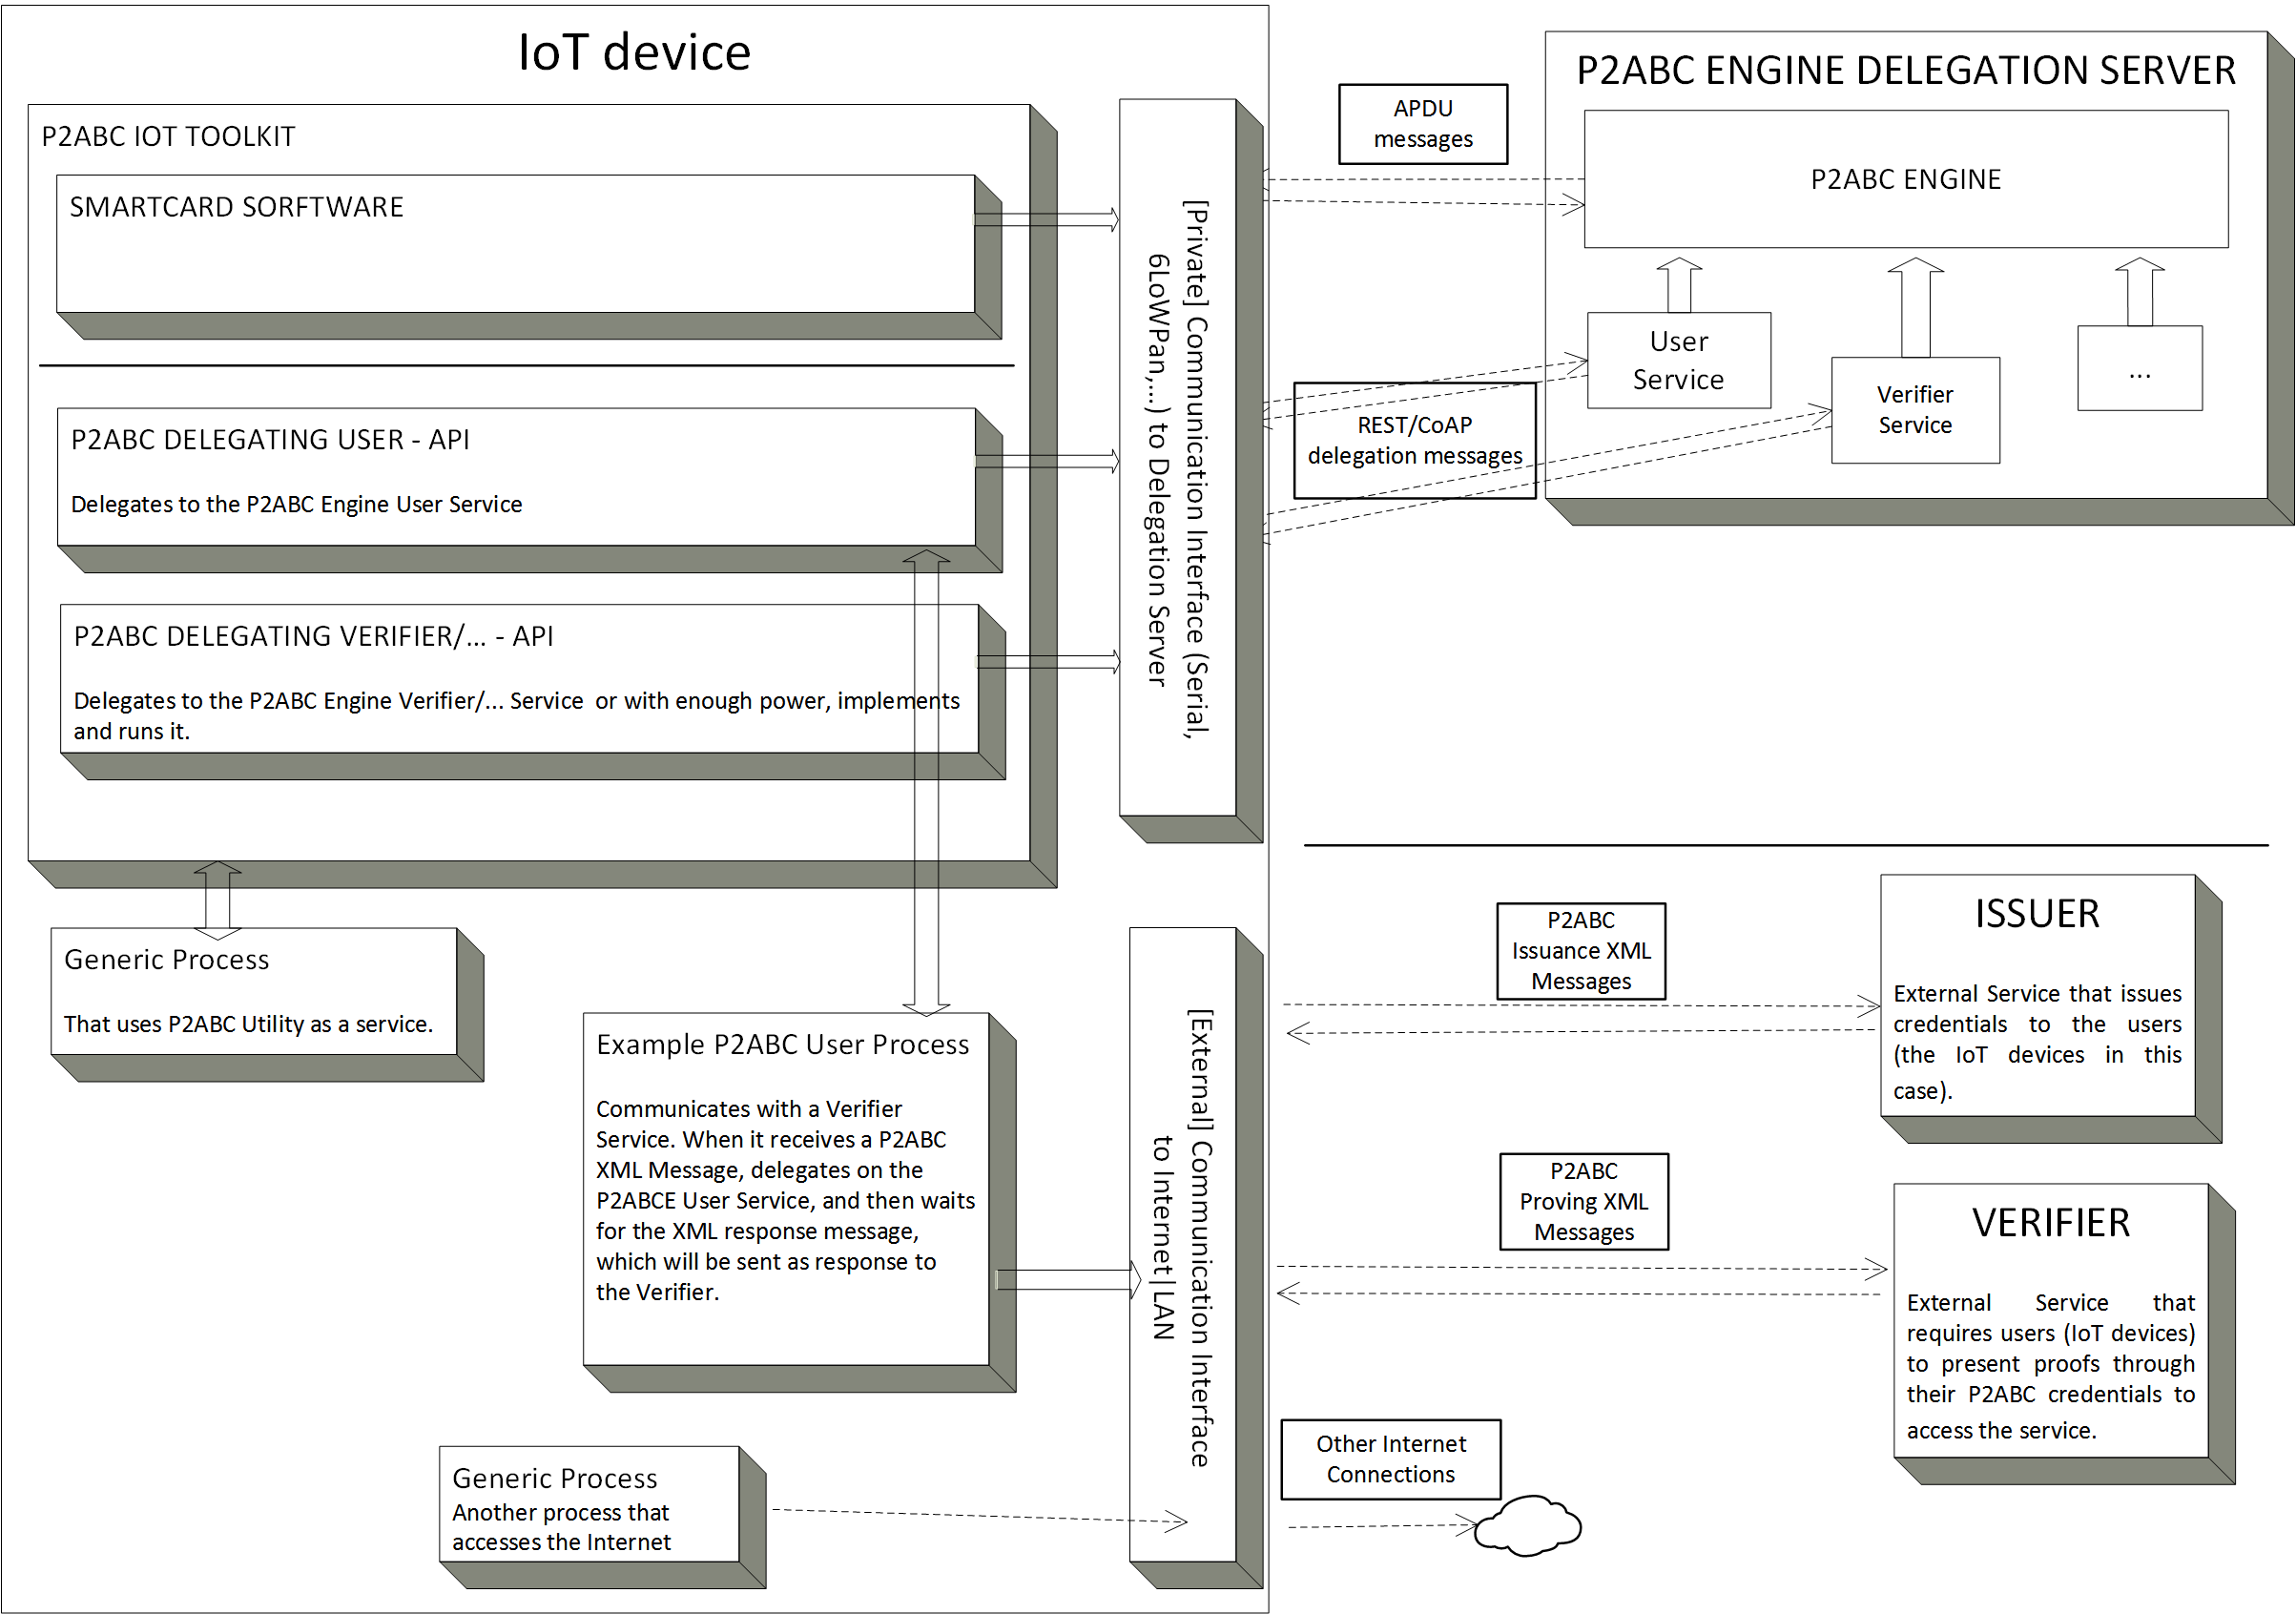
\includegraphics[width=\linewidth]{gfx/P2ABCE-IoT-bw}
	\end{center}
	\caption{IoT in P2ABCE Architecture.}
	\label{fig:P2ABCE-IoT}
\end{figure}

%\begin{figure}[bth]
%	\begin{center}
%		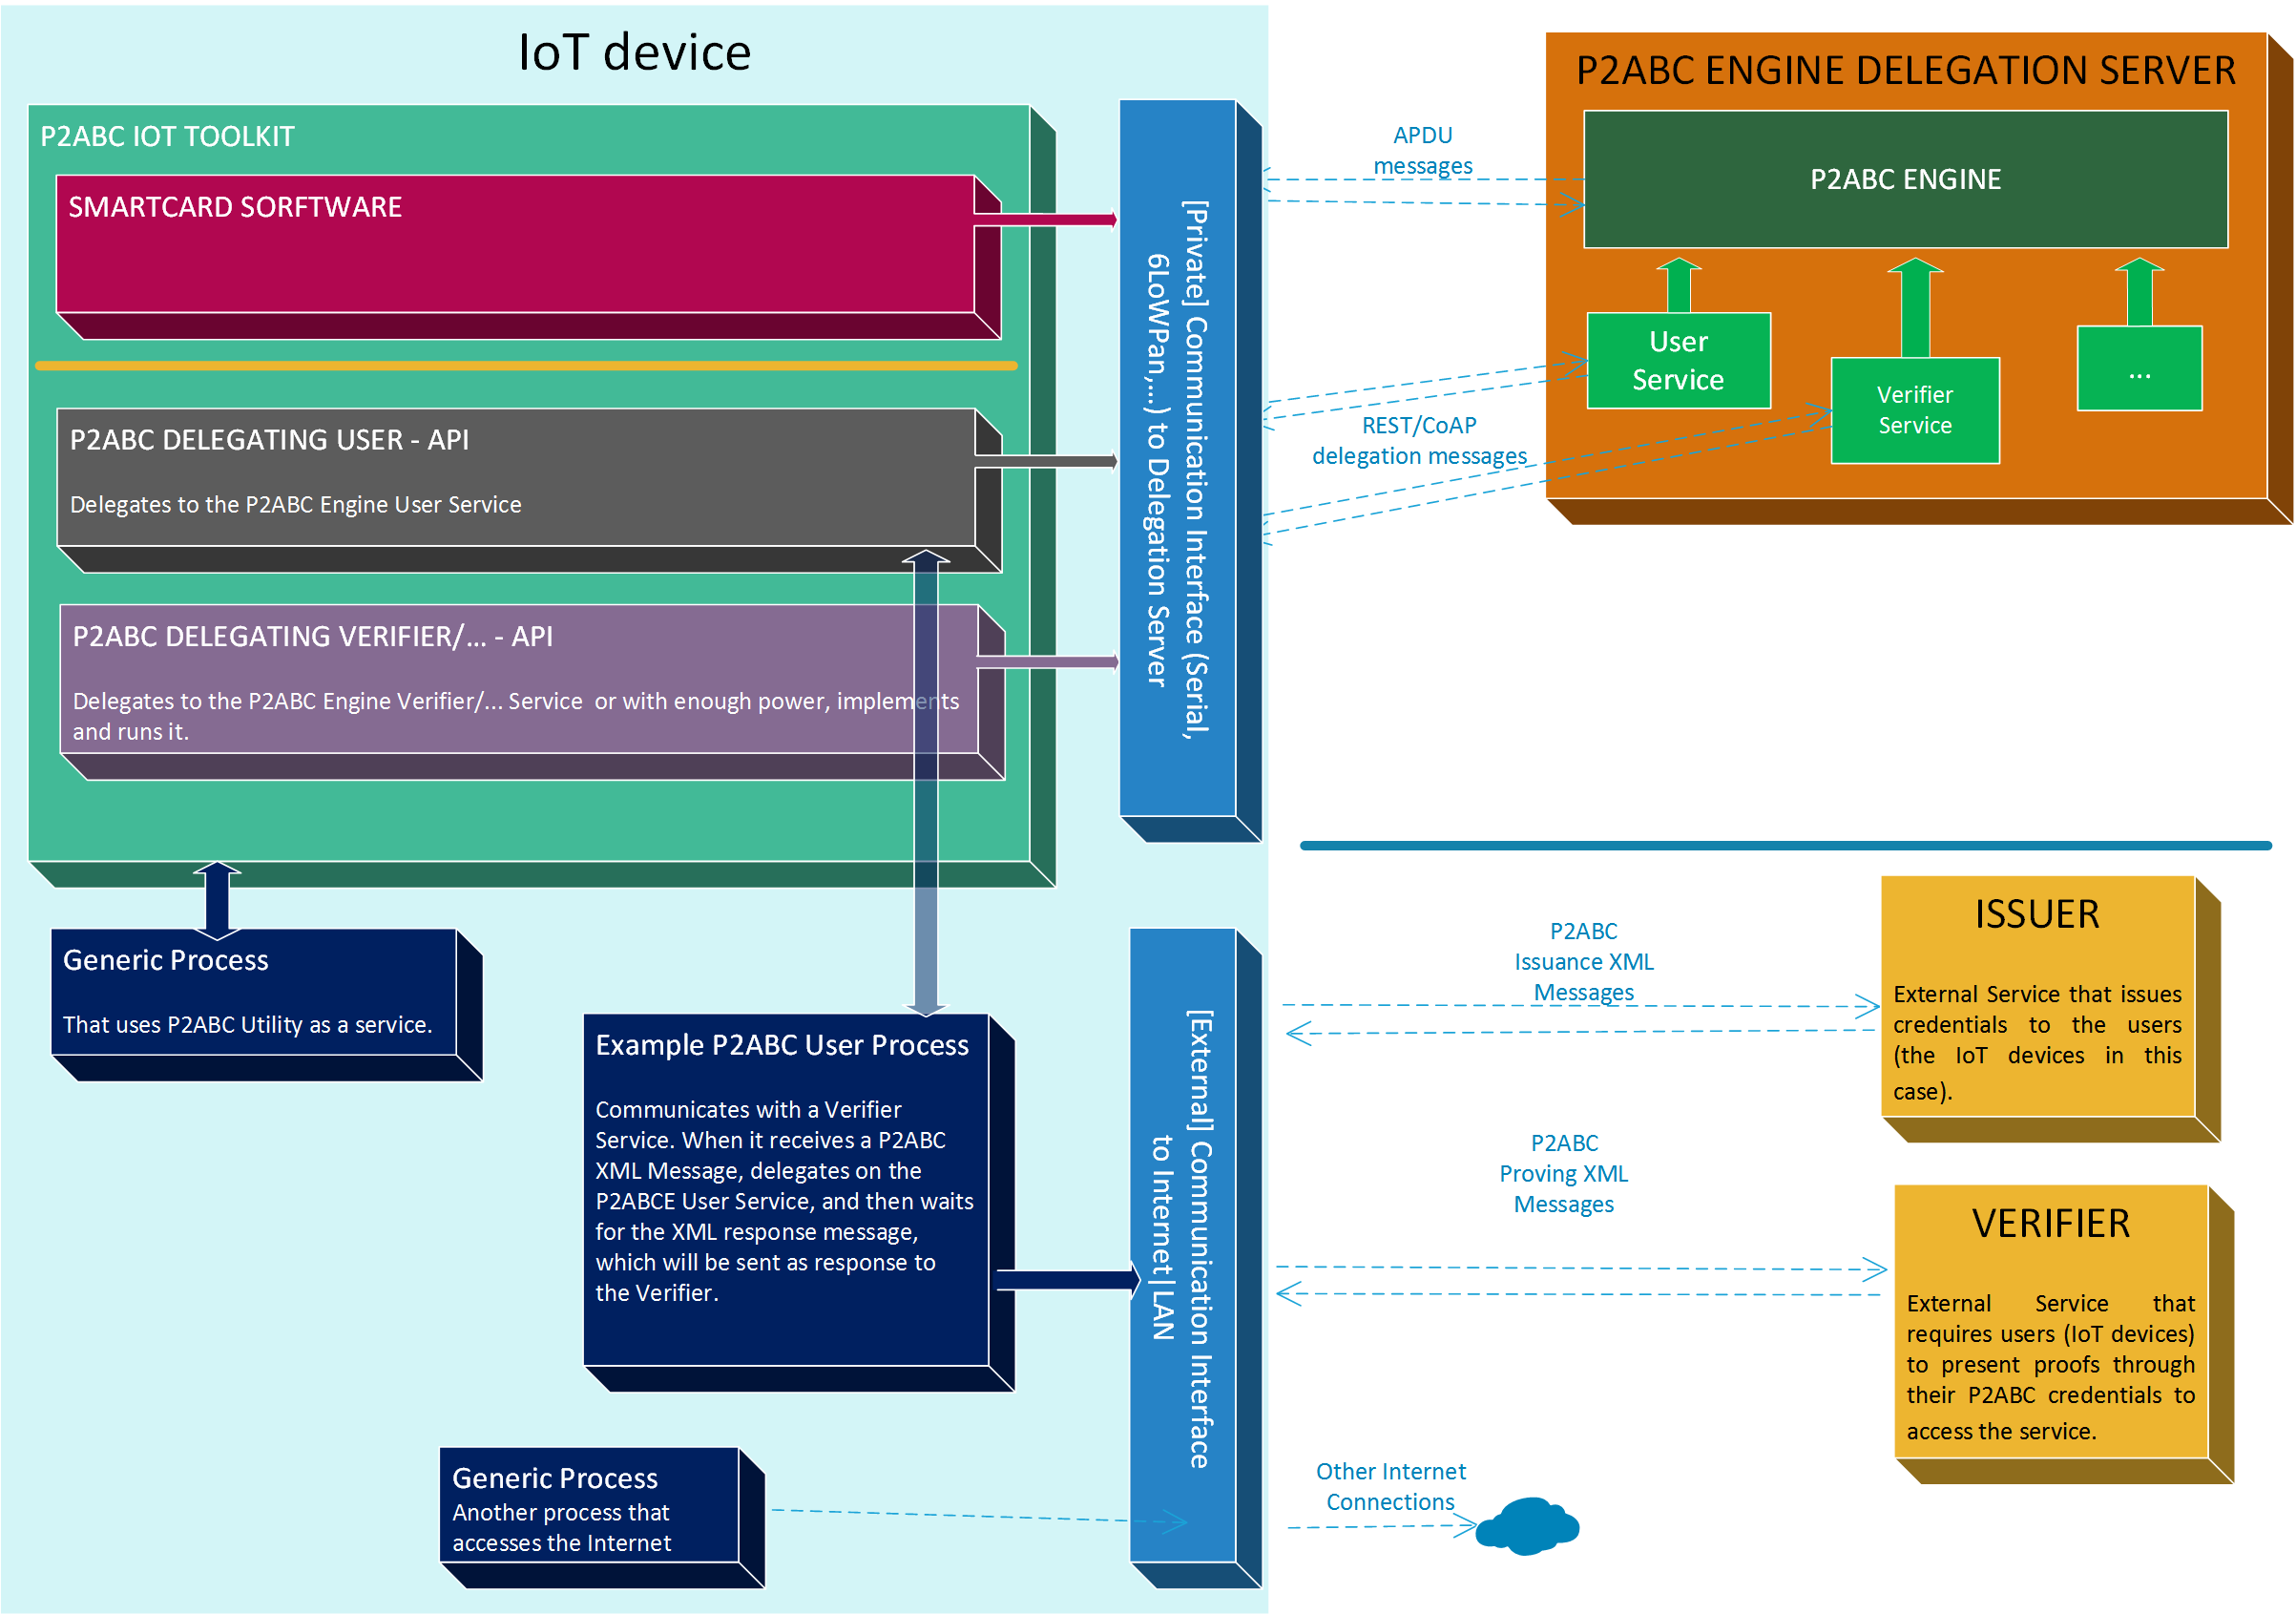
\includegraphics[width=\linewidth]{gfx/P2ABCE-IoT-color}
%	\end{center}
%	\caption{IoT in P2ABCE deployment diagram.}
%	\label{fig:P2ABCE-IoT-color}
%\end{figure}

\hfil


Therefore, the IoT device now has a \textbf{duality} in its functions, because it is the User that starts any interaction with other actors, and it's also the smart card that a P2ABCE server must ask for cryptographic operations. It can also be seen as a \textbf{double delegation}. The IoT device delegates on the external P2ABCE server to manage the protocol, and the P2ABCE server delegates on the IoT, acting now as a smart card, for the cryptography.





\begin{figure}[bth]
	\begin{center}
		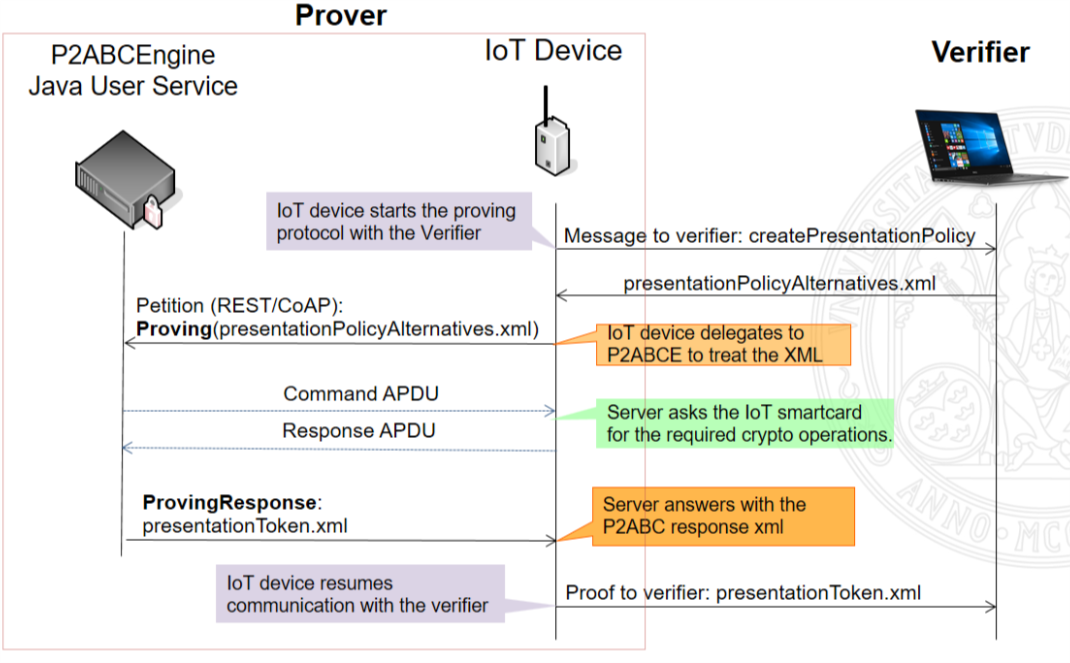
\includegraphics[width=\linewidth]{gfx/DelegationProving}
	\end{center}
	\caption{IoT Delegation in P2ABCE for Proving.}
	\label{fig:DelegationProving}
\end{figure}



\paragraph{PoC Delegation to the P2ABCE Server} \hfil

We now will address each type of delegation: from the IoT device as a P2ABCE actor to the P2ABCE delegation server, and from the server to the smart card in the IoT device.

\hfil

Currently P2ABCE offers multiple REST web services to run different roles in P2ABCE system: User Service, Issuer Service, Verification Service, etc. An application that integrates P2ABCE can make use of this services in the same machine or implement the functionality using the core components written in Java, the same ones the REST services use. Our PoC machine, the Omega2, can make REST calls easily, but other devices may use \ac{CoAP}, and in that case, the P2ABCE REST services should be rewritten to offer CoAP support. The commands needed to delegate to the P2ABCE delegation server will be the same to operate with the REST services. This way, the first issue is solved.

The transmission of the messages will depend on the specific use cases, capabilities and resources available. If the delegation server is connected, for example, through RS-232 serial with the IoT device, and physically inaccessible, in the same way an IoT device on its own would be protected, the communication is simple, and not far away from the Arduino Yun idea of combining two devices, one more powerful but to use only when needed. But if the IoT device and the delegation server are apart, or more than one IoT device delegates to it, then the transmission must be secured. They could use 6LoWPAN to talk to each other (the delegation service could be deployed in the proxy) and then secure communications with existing solutions, like with pre-shared symmetric keys, certificates for authentication and authorization, etc., it depends on each particular deployment.

At the end of the day, this is all about usual security in IoT. Many other studies focus on this matter, so we will assume it can be done, and focus on what's new, P2ABCE in IoT.


\hfil


% TODO: imagen con servicios desplegados/actores en cada máquina


To sum up, our IoT device will act as User (Prover or Verifier) keeping its secrets in a software smart card. When it starts an interaction with other actor of the P2ABCE system (Issuer, Verifier, etc.), the IoT device will delegate with a remote call (using REST in our PoC) to a P2ABCE delegation server, attaching the XML file and the necessary information for the server to send the APDUs to the software smart card (in our PoC using TCP sockets, giving the IP and listening port).



\hfil


This simple design keeps the benefit of a 100\% compatible P2ABCE deployment, and the integration of IoT devices to the P2ABCE ecosystem.

In the future, more functionality currently delegated in the P2ABCE server can be implemented in the IoT device, if its resources allow it. For example, in a M2M environment, where an IoT device can act as User and Verifier, the verification consists on sending a Presentation Policy, and verifying the Presentation Token, which implies less logic than generating it as the User. Therefore, the implementation of the Verifier functionality would reduce significantly the need of a delegation server, but as we said, managing complex XML squemas is not something many IoT devices could do.






\section{Implementation}


\section{IoT Smart Card}

After many design decisions in the process to adapt the original ABC4T Card Lite code to pure C, working over a more usual architecture machine, in this section, we present the current \ac{PoC} code, most important decisions, workflow execution, and future work.

First, let's define what a \textit{more usual architecture} is. If we remember the MULTOS section, the framework gives an application a very specific memory layout and entry and output points of execution, that could be seen as a single process execution machine. Many IoT devices work like a computer, with multiple processes or threads, without pre-loaded data on startup (like the APDU MULTOS loads for the application), a non-volatile memory for data and code, maybe a basic file system in this memory, and RAM with the program's stack, heap, data and code.

Our PoC is tested on a Linux system, and we will give instructions on how to adapt each part to work with other typical IoT systems.
For example, other IoT devices may work like MULTOS and let access variables in non-volatile memory during execution, and in that case, the port should be changed according to these particularities.


\hfil



\subsection{Code structure}


We divide the project in three different sections with the objective of enhancing maintainability, improving future changes, ports, fixes, etc.

The first section is what could be called as the core of the smart card, the second one the interface for the tools the core need and may depend on the platform, and finally third party libraries, that in may be empty if the interfaces implementation doesn't need any.


In our PoC we used CMake to manage the project, due to the cross-compilation tools, integration with multiple IDEs and tests.


%\begin{figure}[bth]
%	\begin{center}
%		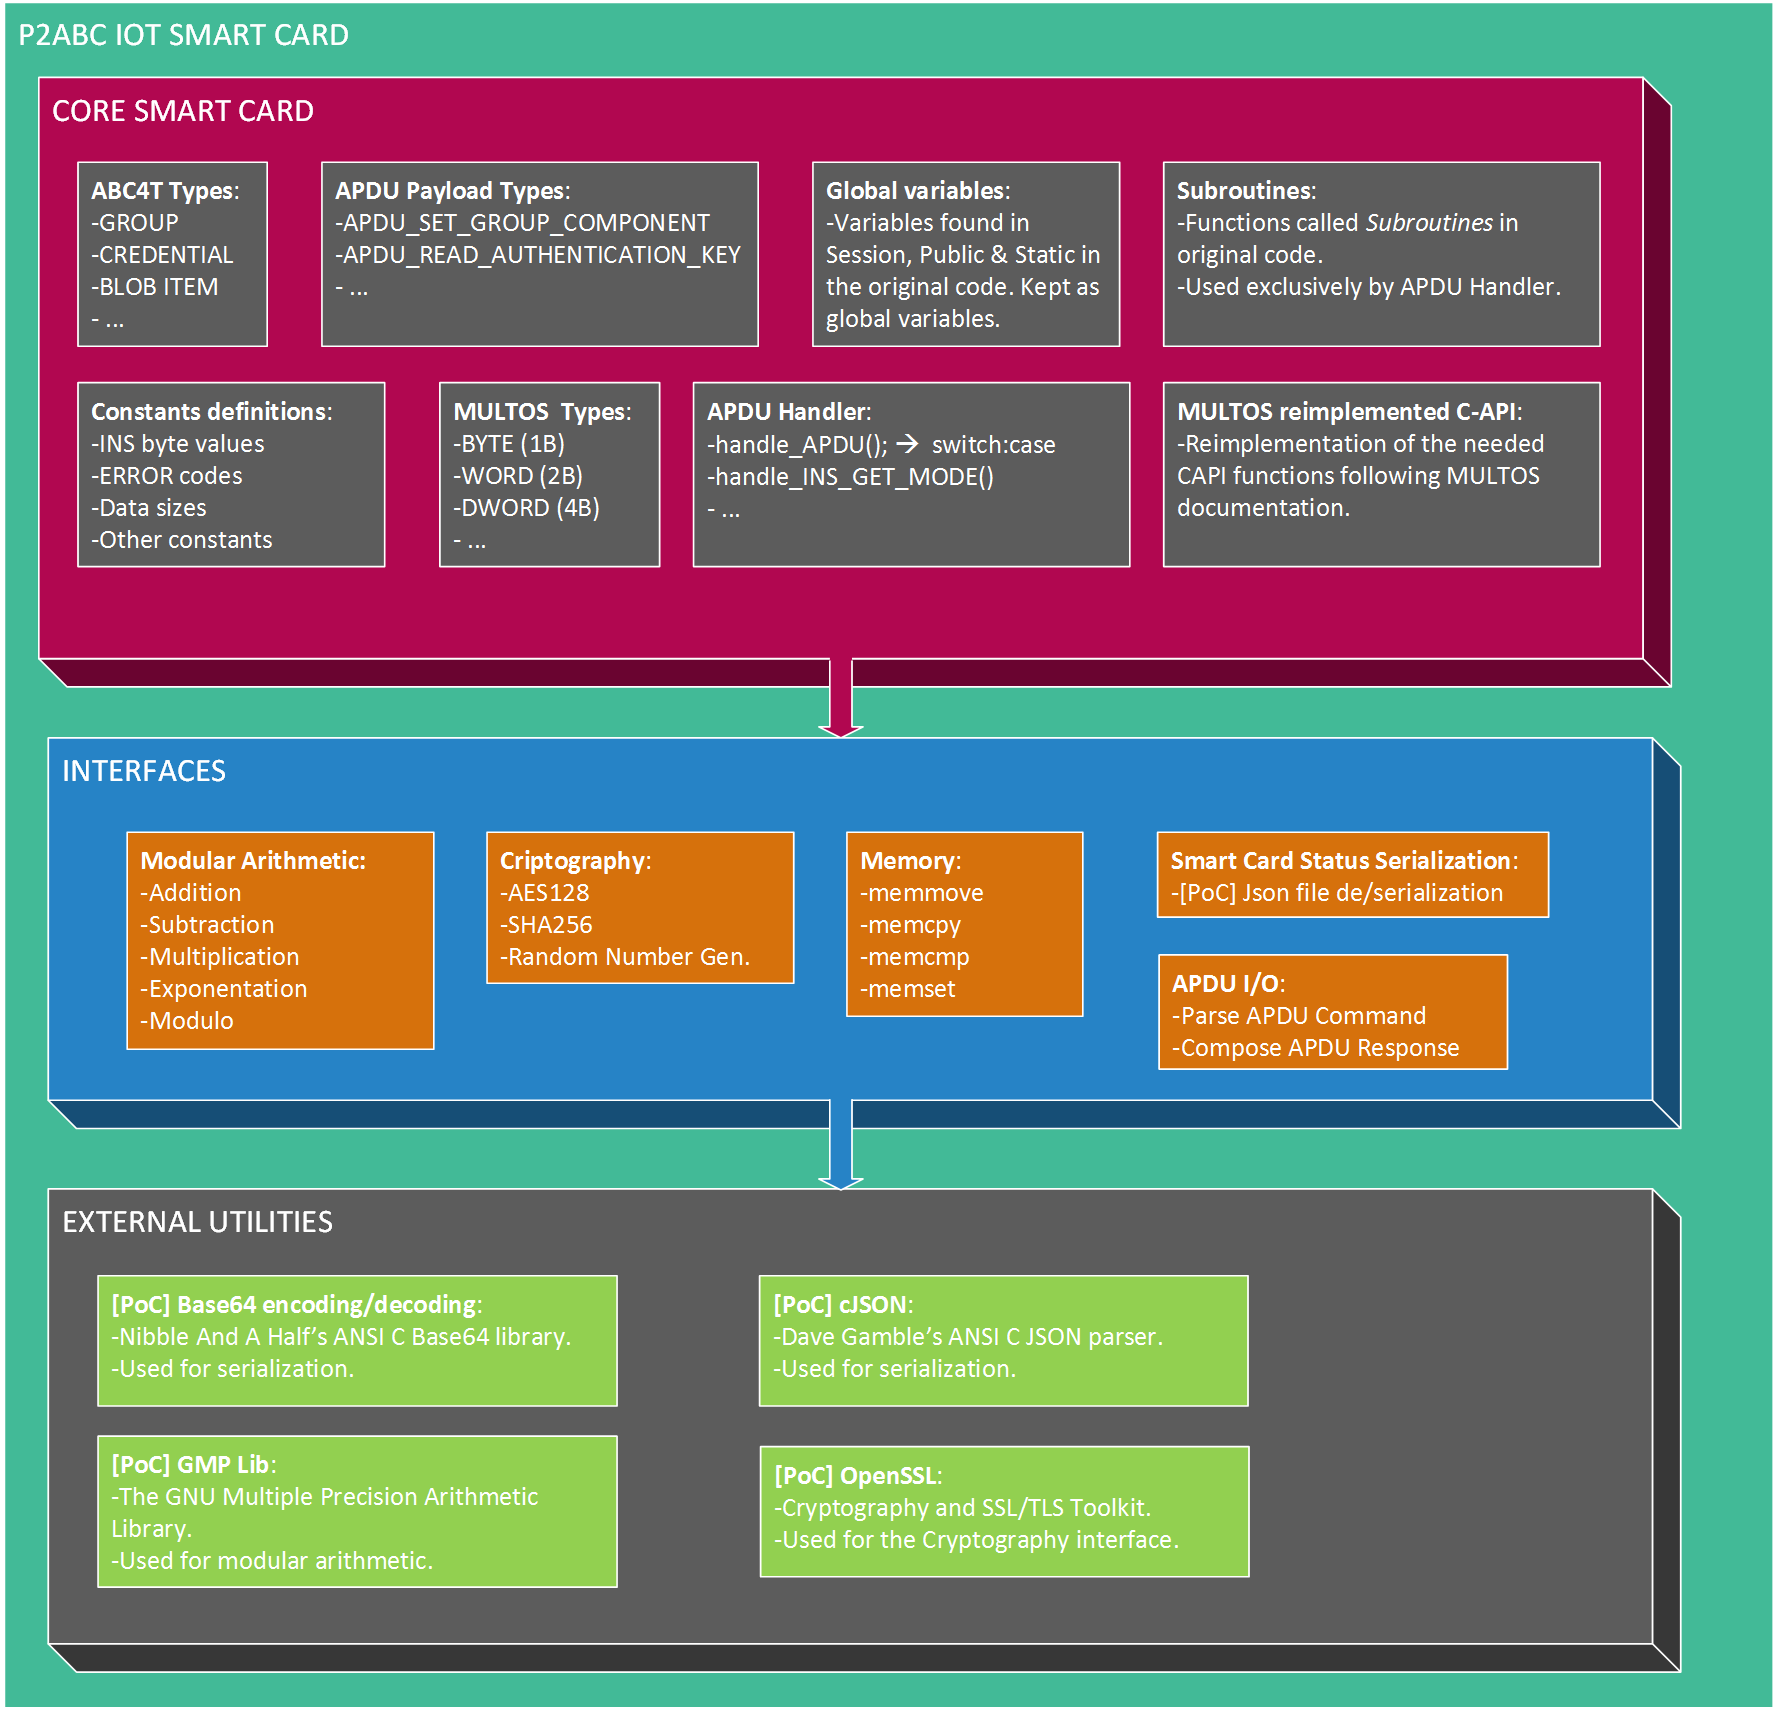
\includegraphics[width=\linewidth]{gfx/IoTCScomponents-color}
%	\end{center}
%	\caption{IoT Smart Card Code Structure.}
%	\label{fig:IoTCScomponents-color}
%\end{figure}

\begin{figure}[bth]
	\begin{center}
		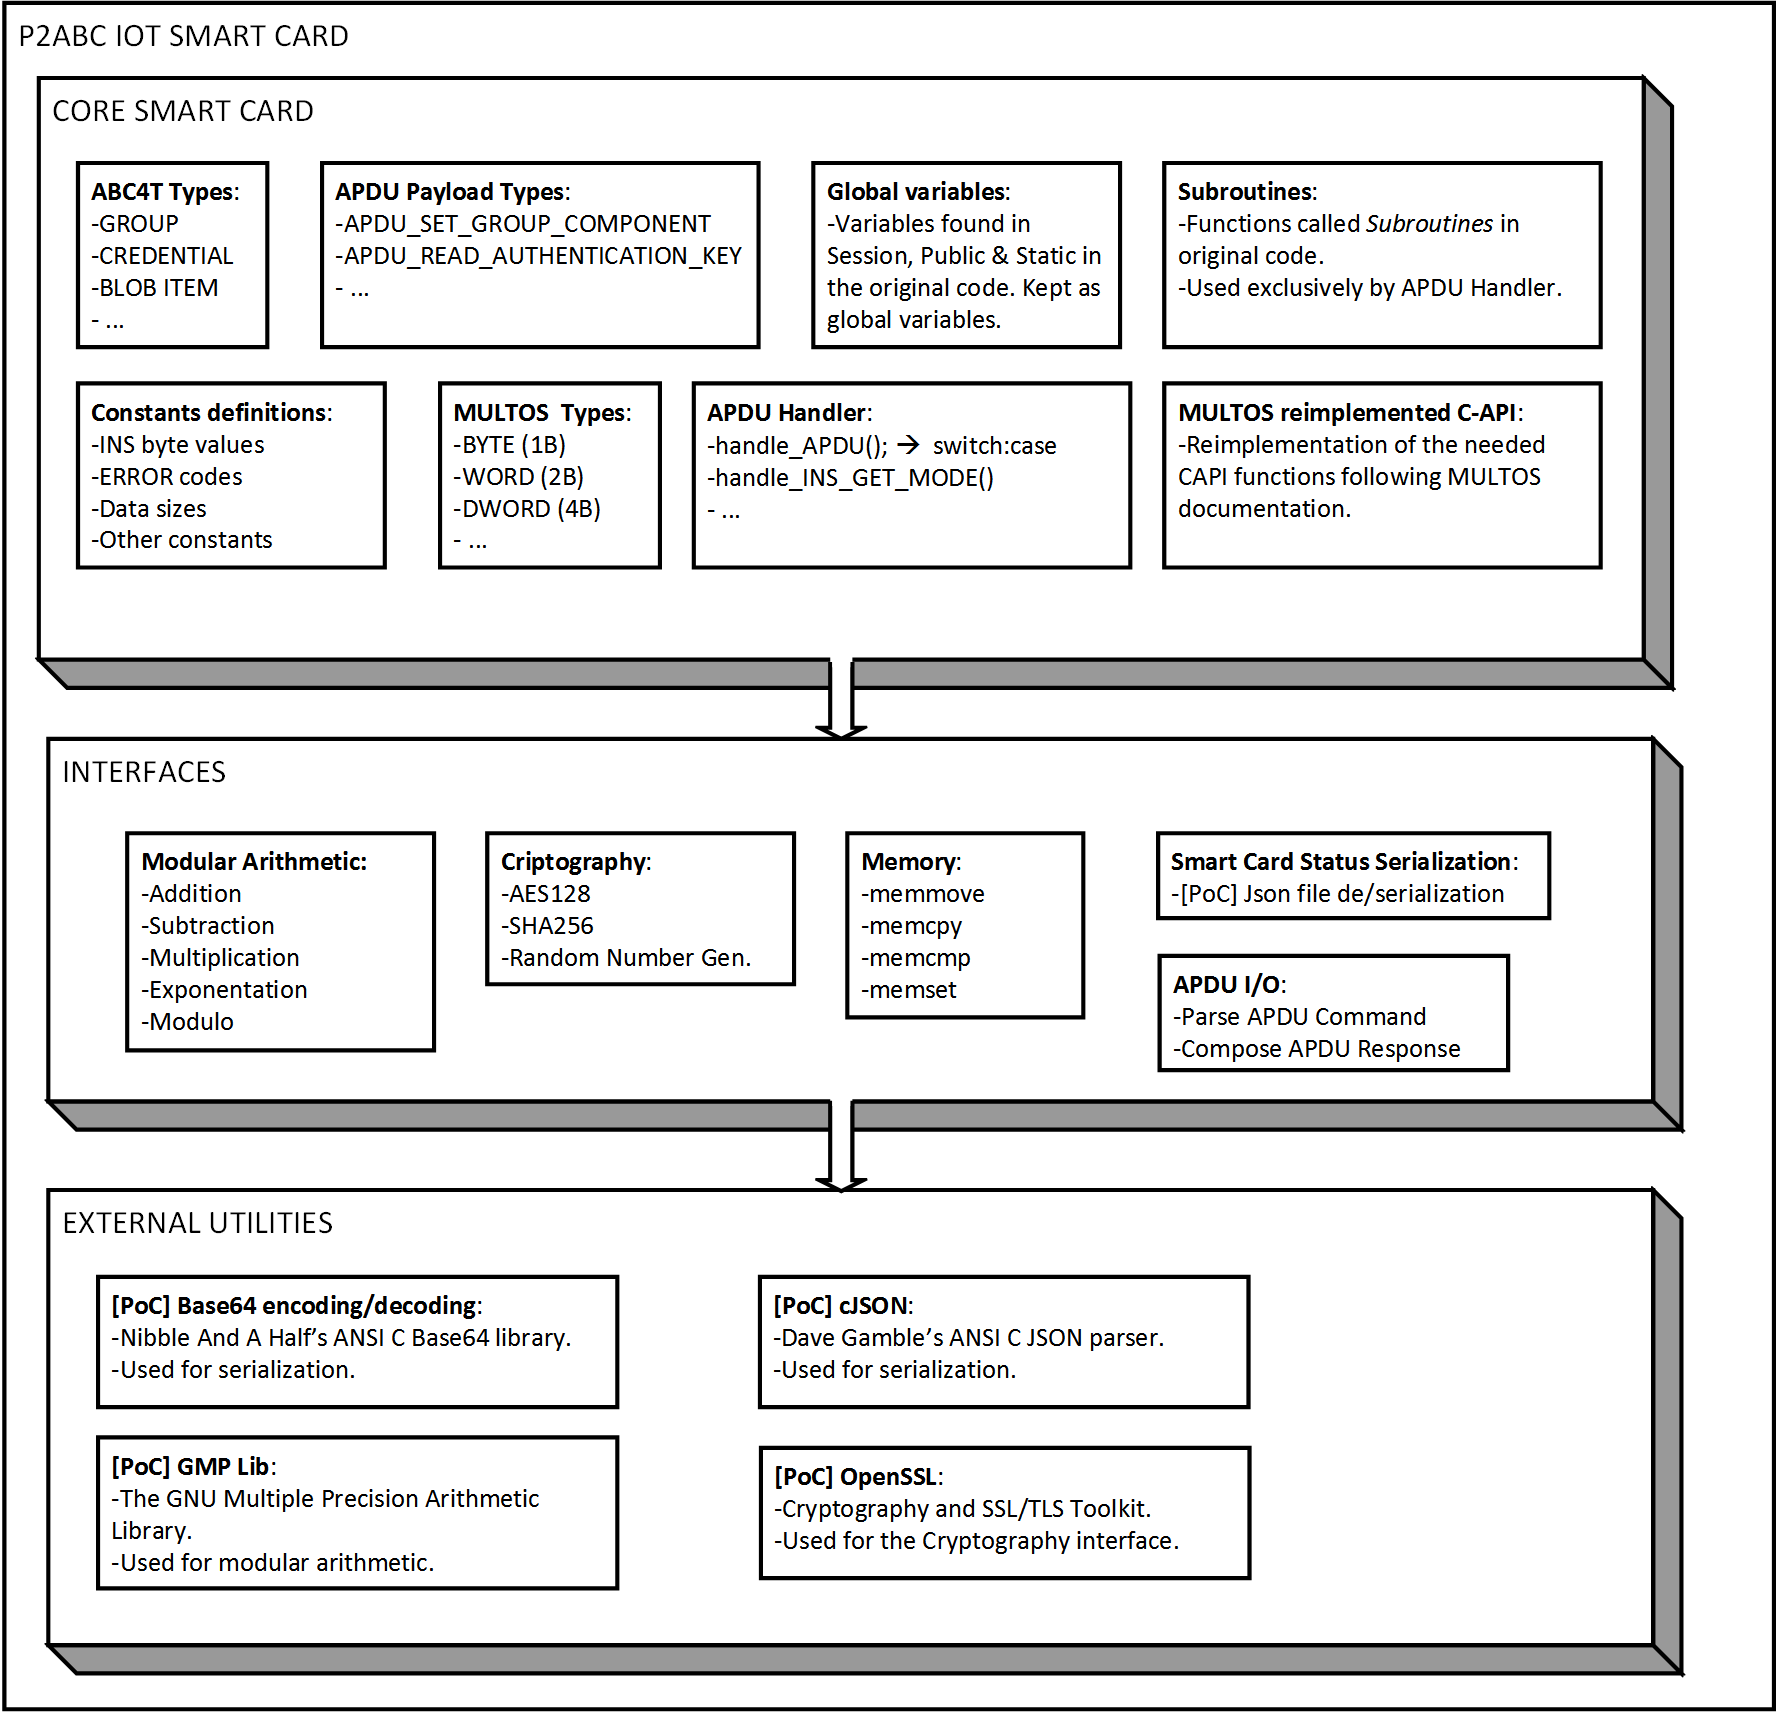
\includegraphics[width=\linewidth]{gfx/IoTCScomponents-bw}
	\end{center}
	\caption{IoT Smart Card Code Structure.}
	\label{fig:IoTCScomponents-bw}
\end{figure}


\hfil

\paragraph{Core smart card}

The smart card logic lies in this section, the concepts of APDU Commands, what instructions are defined in P2ABCE smart cards and how to process them and generate proper APDU Responses.

Changes in the APDU protocol for P2ABCE must be done here, independently of the target platform.

After refactoring the original ABC4Trust Card's code, most of it fell in what we will call the core of the smart card.

All types and variable definitions and the APDU handling is done in this code.
However, the ABC4Trust's code depended on the MULTOS C-API for the input/output of data, modular arithmetic, and even AES128 and SHA256 cryptography.

A characteristic of MULTOS C-API is that every function name starts with \textit{multos}, but as we said, the \textit{main.h} file implemented equivalent functions to some available in \textit{multos.h}. Our first step was to replace the \textit{main.h} functions for the standard ones in the C-API. Then, we implemented, following the C-API documentation, the functions from \textit{multos.h} (only the used ones) changing their names from \textit{multosFoo()} to \textit{mFoo()} for readability and emphasize that they were no longer from MULTOS.

Future changes in the code may refactor it so there's no longer need for the MULTOS framework functions.


\paragraph{Interfaces}

To implement MULTOS functions, we needed to use some libraries, so we defined a facade to isolate the implementation of the core smart card from our different options, that could vary depending on the hardware or the system used by the IoT device.

The use of a facade lets us, for example, change the implementation of modular arithmetic with a hardware optimized version, or a future more lightweight library, or our very own software implementation using the same data types that the core uses, minimizing the data transformations needed.

Taking a step forward, we make the core smart card totally independent of any library, only on our interfaces. This means that typical C libraries, like the standard \textit{stdlib.h}, or  \textit{string.h} are also behind the facade, in case some IoT system doesn't support them. The main goal we go after with this decision is that future developers adapting the code to a specific platform need to make no change to the \textit{core smart card}'s code, only to the interfaces implementation.



\paragraph{External utilities}

If the IoT system offers well tested libraries that could aid in the interfaces implementation, or we simply found a pure C implementation for the task, these third party libraries belong to this section.

In our PoC, we use two ANSI C libraries, for base64 and JSON, and two shared libraries available in as packages in LEDE, GMPLib and OpenSSL. The last two libraries offer more functionality than we need, hence, it's desired in a production code to implement \textit{Modular Arithmetic} and \textit{Cryptography} interfaces with more lightweight alternatives.

For example, Atmel's ATAES132A \citep{ATAES132A}
\marginpar{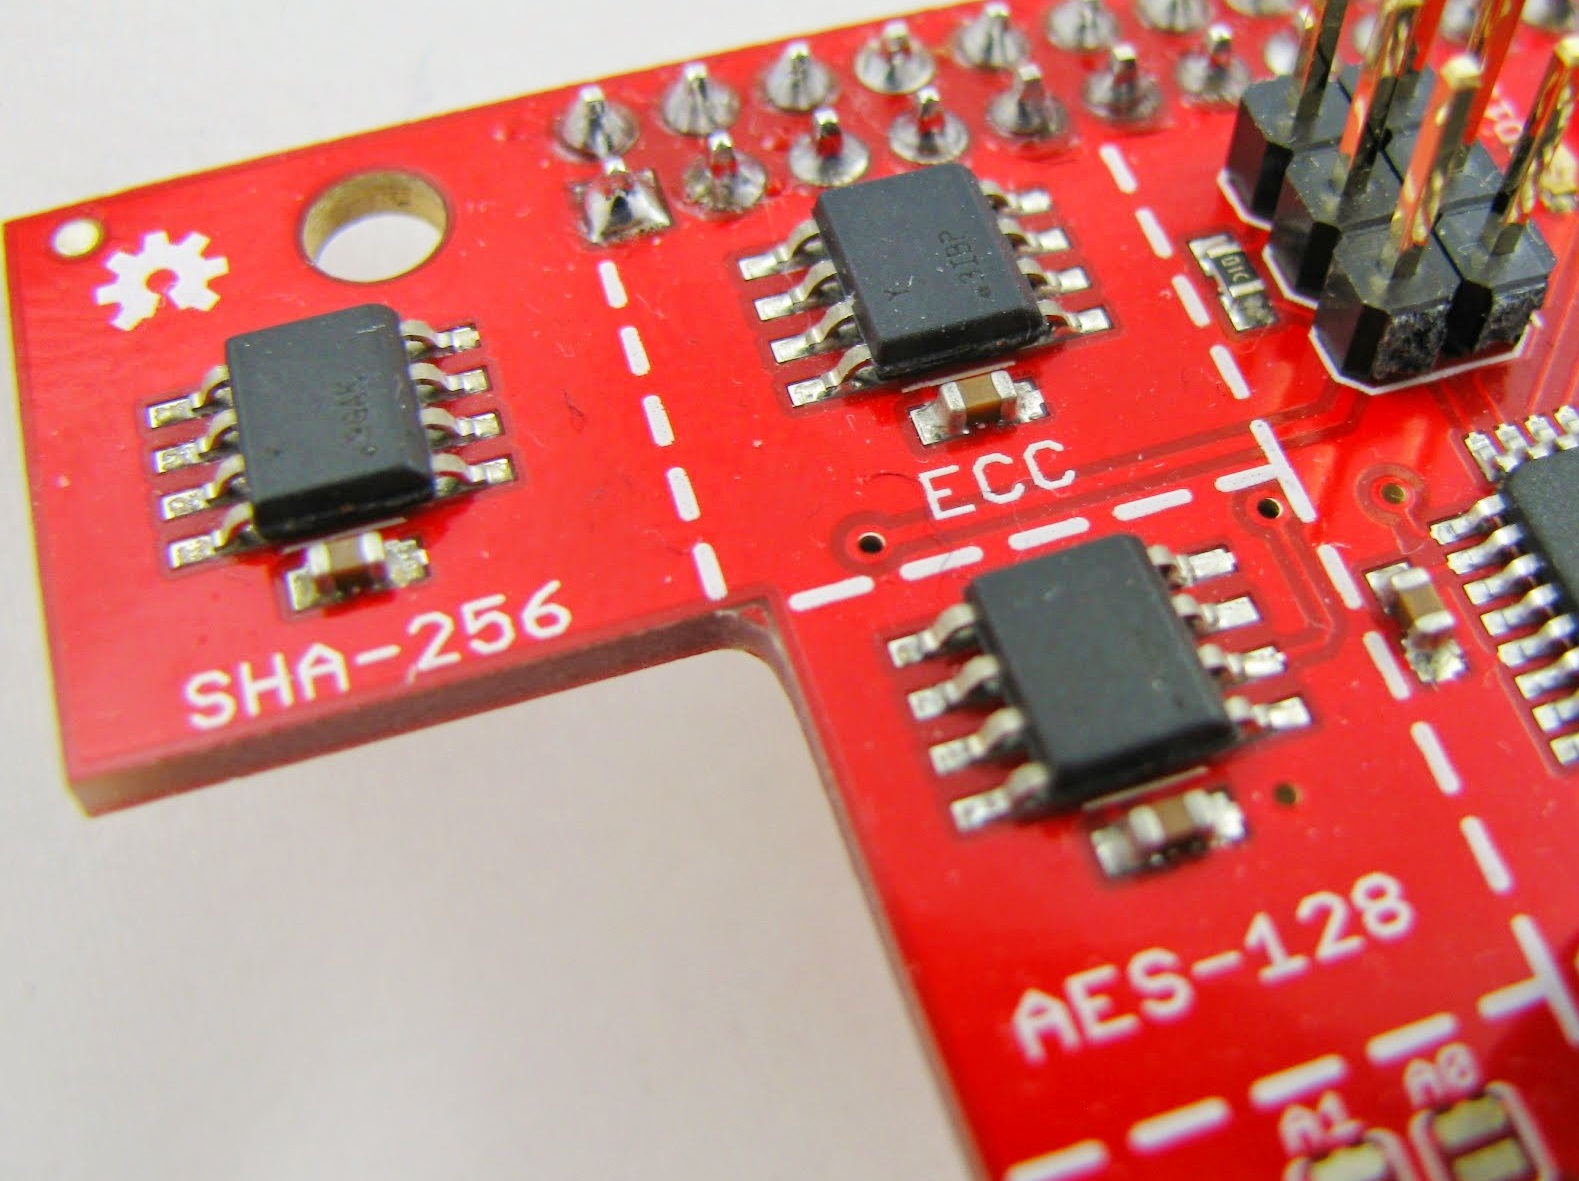
\includegraphics[width=0.9\linewidth]{gfx/atmel} \\ Atmel's cryptography chips.}
offers a serial chip for secure key storage, AES128 execution and random number generation. Another serial chip like ESP8266 offers WiFi connectivity, typically used with Arduino, and can also perform AES encryption. For random number generation, a technique used with Contiki devices is to read from sensors aleatory data and use it as seed. All these alternatives depend on the target device, but are all valid. The \textit{interfaces} and \textit{external utilities} sections allow for a clean and fast port of the code.


\subsection{PoC Workflow}

% PoC BIOSC : TCP sockets, JSON serialization

% PoC IoT javax.smartcardio : protocolo de 2 bytes + APDU

% 1. Boot: deserialize sc status
% 2. Listening: open tcp socket
% 3. The IoT device delegates on the P2ABCE for some task and sends the IP and Port of the IoT Smart Card.
% 4. An APDU Command arrives : read in 2 bytes the length of the apdu and 


In a real deployment, we would offer a full library with an API to other processes to delegate on the P2ABC Engine, that automatizes the listening and security, that we presented in the deployment diagram \textbf{TODO:ref-img} as the \textit{P2ABCE IoT Toolkit}.

But to test the IoT smart card, we use the \textit{curl} command for REST delegation calls and the BIOSC (Basic Input Output Smart Card) for APDU communication.

To transmit the APDU messages in our PoC we use a simple protocol, consisting in one first byte for the instruction: receive an APDU Command or close the connection. In the first case, then we read two header bytes with the length of the APDU Command or Response to receive, followed by those APDU bytes. The message is sent over TCP for a reliable transmission (concept of session, packet retransmission, reordering, etc.).

We lack of any security (authentication and authorization) that a real system should implement. It is vital to authenticate the delegation service, to authorize it to make APDU Commands, and the same with the IoT device, to prevent attacks. This belongs to \textit{usual} security, as we already said, and for that reason it's not in the PoC.

\paragraph{P2ABCE REST Delegation}


The only P2ABCE Service that needed to be modified was the User Service. We added the REST call

\begin{center}
	\textit{/initIoTsmartcard/{issuerParametersUid}?host=\&port=}
\end{center}

where we communicate the P2ABCE server that a IoT Smart Card is accessible via \textit{host} and \textit{port}. Then a new \textit{HardwareSmartcard} object is stored in the P2ABC Engine, but instead of the \textit{javax.smartcardio} Oracle's \textit{CardTerminal} implementation, we use our \textit{IoTsmartcardio} implementation for the \textit{HardwareSmartcard} constructor.

The rest of P2ABCE code is unchanged and will work as if a real smart card was in use. \textit{IoTsmartcardio} implementation will transmit the APDUs through the TCP socket with the format mentioned.


\hfil

Our test consists on the tutorial available in P2ABCE's repository. From the Omega2's terminal we run \textit{curl} commands to send REST petitions. For example:

\begin{verbatim}
$ curl -X POST --header 'Content-Type: text/xml'
'http://localhost:9200/user/initIoTsmartcard/http%3A%2F%2
Fticketcompany%2FMyFavoriteSoccerTeam%2Fissuance%3Aidemix
?host=192.168.3.1&port=8888'
\end{verbatim}

The IoT device will only manage XML as data files to exchange between the third party actor and the P2ABCE delegation service, without parsing them.

After a REST call to the User Service, the P2ABC Engine will talk to the IoT smart card process.

\paragraph{APDU transmission with BIOSC}

% TODO : diagrama del software

Before sending the REST message, the Omega2 must be listening in the specified port. At start up, BIOSC reads from a JSON file the status of the smart card (credentials in the BLOB, private keys, PIN and PUK codes, etc.), then opens the TCP socket and listens in a loop.

When the delegation server sends an APDU Command following the simple protocol, BIOSC stores in a byte array the APDU Command bytes and calls the \textit{handle\_APDU} function in \textit{Core Smart Card}.


The \textit{APDU\_handler} will parse the APDU bytes and check both CLA and INS bytes. For each possible INS the is a function that must always finish calling either \textit{mExit()} or \textit{output\_large\_data()}.

The \textit{mExit} function is the reimplementation of MULTOS C-API exit functionality, that finishes the application execution returning to the MULTOS OS, that will send the APDU Response bytes to the terminal. This led in the original ABC4Trust Card's code to some tricky situations. Imagine a function that ends with an if-else expression. Many times we save a line writing something like

\begin{verbatim}
if(condition)
return a;
return b;
\end{verbatim}

instead of the complete

\begin{verbatim}
if(condition)
return a;
else
return b;
\end{verbatim}

This is a swift example of what the \textit{multosExit} function led to, because it is called in both the \textit{switch-case} processing the APDU instruction, and the \textit{Subroutines}. For example, the PIN code check was programmed in a way every reason to fail finished the application execution, with different error codes. Another example, checking if a credential is stored, if not, fail and exit inside the \textit{readBlob} subroutine.

In our standard architecture machine, if we call a subroutine, it must end, and return the control to the handling function, and so the \textit{APDU\_handler} must return to the listening loop of BIOSC.

Having all that in count, the \textit{mExit} function is not implemented as the documentation specifies, but only saves the smart card status serializing it in the JSON file again, and once it's saved, parses the APDU Response and sends it to the socket.

The \textit{output\_large\_data} function is a tool used in MULTOS smart cards that don't support Extended APDUs. The APDU Command handler saves in a buffer the data to send, and its size. Then, \textit{output\_large\_data} will manage the buffer expecting future GET RESPONSE commands from the P2ABCE server.

A future change to the project may include support for Extended APDUs, avoiding the use of multiple GET RESPONSE. To do this, the \textit{output\_large\_data} function and the \textit{IoTsmartcardio} implementation of \textit{javax.smartcardio} must support the feature.


% TODO -Sequence diagrams.




